L'article \cite{Vardhan04} se concentre sur un automate plus général : l'automate à files. Les automates à files sont plus complexes que les ADF. Les langages définis par ceux-ci sont plus complexes que les langages réguliers mais toujours dans l'espace défini par $\Sigma^*$. La figure \ref{fig:lrl} propose une intuition des langages définis par les automates à files.


\begin{figure}[H]
  \centering
  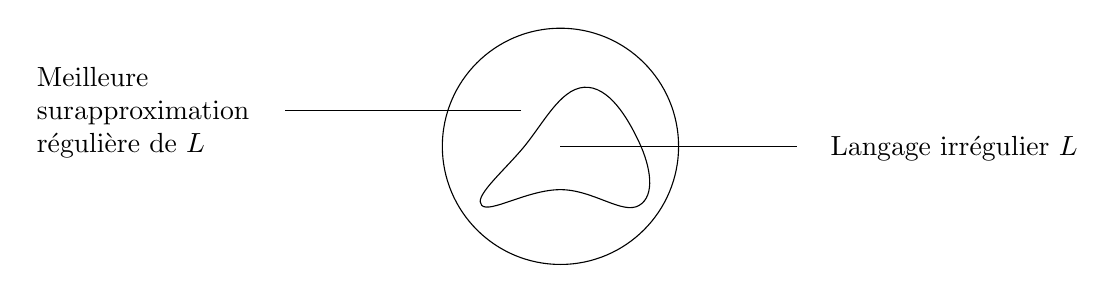
\begin{tikzpicture}[>=latex]
        \draw plot [smooth cycle, tension=0.75] coordinates {
          (0.5,0)
          (1.5,0.2)
          (2.5,0)
          (2.5,0.8)
          (1.8,1.5)
          (1.0,0.7)
        };
        \draw (1.50,0.75) circle (1.5);
        \draw (1.5,0.75) -- (4.5, 0.75);
        \draw (1,1.2) -- (-2, 1.2);

        \node at (6.50,0.72) {Langage irrégulier $L$};
        \node[align=left] at (-3.8, 1.18) {Meilleure\\ surapproximation \\ régulière de $L$};
  \end{tikzpicture}
  \caption{Relation entre langage régulier et langage irrégulier}\label{fig:lrl}
\end{figure}

Ainsi, de nouveaux langages peuvent être définis de façon plus précise. Leur puissance expressive est équivalente aux machines de Turing. Cela a un coût : pour certains problèmes il n'existe pas de réponse générale ou si celle-ci existe elle prend un temps exponentiel à construire.


C'est le cas de la question de sécurité des automates à files dans ce mémoire. Cependant, le chapitre \ref{lever} décrit comment une solution peut-être construite pour tout un ensemble d'automates à files, permettant de se prononcer sur un ensemble plus large que les langages régulier. L'automate à file est dès lors un outil pertinent pour élargir l'ensemble des langages pour lesquels il est possible d'étudier la sécurité.

Cette section se divise en une première partie \ref{fifo:def} donnant une définition formelle des automates à files et un exemple ainsi qu'une seconde partie \ref{fifo:trans} sur les systèmes de transitions, représentation potentiellement infinie des différentes configurations d'un automate à files. Finalement, la section \ref{fifo:lang} donne une définition formelle de ces nouveaux langages représentés par des automates à files.



% ██████  ███████ ███████
% ██   ██ ██      ██
% ██   ██ █████   █████
% ██   ██ ██      ██
% ██████  ███████ ██

\subsection{Définition}\label{fifo:def}
\begin{definition}
  Un \emph{automate à files} \fifo est défini comme suit :
  \begin{itemize}
    \item $Q$ est un ensemble fini d'\emph{états de contrôle}
    \item $C$ est un ensemble fini de \emph{canaux}
    \item $\Sigma$ est un alphabet
    \item $q_0 \in Q$ est l'\emph{état de contrôle initial}
    \item $\Theta$ est un ensemble fini de \emph{noms de transitions}
    \item $\delta$ est la \emph{fonction nommante}. $\delta : \Theta \rightarrow Q \times ((C \times \{?,!\} \times \Sigma) \bigcup \{\tau\}) \times Q$. Un nom de transition $\theta$ correspond à une transition de la forme $\delta(\theta)=(p,\text{"action"},q)$. Cette action a une des trois formes suivantes :
    \begin{itemize}
      \item $c!m$ : C'est une action d'envoi. Le symbole $m\in\Sigma$ est ajouté en fin de canal $c$.
      \item $c?m$ : C'est une action de réception. Le symbole $m\in\Sigma$ est consommé en début de canal $c$.
      \item $\tau$ : C'est une action interne. Aucun canal n'est modifié.
    \end{itemize}
  \end{itemize}
\end{definition}


% ███████ ██   ██
% ██       ██ ██
% █████     ███
% ██       ██ ██
% ███████ ██   ██


\begin{example}
  Soit un automate à files $F$ donné à la figure \ref{fig:fifo1}.

  \begin{figure}[H]
    \centering
    \begin{tikzpicture}[->,>=stealth',shorten >=1pt,auto,node distance=2.5cm, semithick, bend angle=10]

      \tikzstyle{every state}=[circle]

      \node[initial,state] (A)                    {$q_0$};
      \node[state]         (B) [above right= 1cm and 3 cm of A] {$q_1$};
      \node[state]         (C) [below right= 1cm and 3 cm of A] {$q_2$};
      \node[state]         (D) [above right= 1cm and 3 cm of C] {$q_3$};

      \path
      (A) edge node {$\theta_1(a!0)$} (B)
      (A) edge node[below left] {$\theta_2(a!1)$} (C)
      (B) edge node {$\theta_4(a?0)$} (D)
      (B) edge[loop above] node {$\theta_3(b!1)$} (B)
      (C) edge node[below right] {$\theta_6(a?1)$} (D)
      (C) edge [loop below] node{$\theta_5(b!0)$} (C)
      (D) edge node[above] {$\theta_7(b?0)$} (A)
      ;
    \end{tikzpicture}
    \caption{Automate à files $F$}\label{fig:fifo1}
  \end{figure}

  On retrouve bien la définition d'un automate à files \fifo avec :
  \begin{itemize}
    \item $Q=\{q_0,q_1,q_2,q_3\}$
    \item $C=\{a,b\}$
    \item $\Sigma=\{0,1\}$
    \item $q_0\in Q$
    \item $\Theta=\{\theta_1, \theta_2, \theta_3, \theta_4, \theta_5, \theta_6\}$
    \item $\delta$ associant à chaque $\theta_i$ un triplet état/action/état telle que l'action est représentée entre parenthèses à côté du nom de transition associé
  \end{itemize}
\end{example}


\todo{exemple trace pour demo algo appartenance : $\bar{\theta_2}\bar{\theta_5}\bar{\theta_5}\bar{\theta_1}t_{q_0}$}





\subsection{Système de transitions}\label{fifo:trans}


Un automate $F$ défini un \emph{système de transitions} \tsys. $\mathcal{T}$ est l'objet qui permet de passer d'un \emph{état} à un autre.

En effet, il existe les états de contrôles $q\in Q$, mais les états au sens d'un automate à files sont de forme $s \in S=Q\times(\Sigma^*)^C$. En particulier, $s=(q,w)$ avec $q\in Q$ un état de contrôle et $w\in (\Sigma^*)^C$ est un vecteur qui fait correspondre à chaque canal $c\in C$ un mot $w[c] \in \Sigma^*$ représentant le contenu de ce canal. Intuitivement, un état $s$ est composé d'un état de contrôle et du contenu des différents canaux.

De plus, la \emph{fonction de transition} $\rightarrow:S\times\Theta\rightarrow S$ associe un état $s\in S$ et un nom de transition $\theta\in\Theta$ à un état $s'\in S$.

$\mathcal{T}$ respecte trois règles, correspondant chacune à un des types d'actions pouvant être associées par la fonction nommante. En plus de la notation $w[c]$, celles-ci utilisent la notation $w[c\mapsto c']$ signifiant $w$ à l'exception du canal $c$ dont le contenu a été remplacé par le mot $c'$.
\begin{itemize}
  \item Si $\delta(\theta)=(p,c?m,q)$ alors $(p,w)\xrightarrow{\theta}(q,w')$ si et seulement si $w=w'[c\mapsto mw'[c]]$
  \item Si $\delta(\theta)=(p,c!m,q)$ alors $(p,w)\xrightarrow{\theta}(q,w')$ si et seulement si $w'=w[c\mapsto mw[c]]$
  \item Si $\delta(\theta)=(p,\tau,q)$ alors $(p,w)\xrightarrow{\theta}(q,w')$ si et seulement si $w=w'$
\end{itemize}

\begin{example}

  Reprenons l'automate à files $F$ de la figure \ref{fig:fifo1}. Un système de transitions $\mathcal{T}$ peut lui être associé.

  Considérons le mot $w=[\epsilon,\epsilon]$ où le premier élément du vecteur est le contenu du canal $a$ et le second celui du canal $b$.
  Dans cet exemple, comme $\delta(\theta_1)=(q_0,a!0,q_1)$, alors $(q_0,w)\xrightarrow{\theta_1}(q_1,w')$. Dans ce cas, $w'=[0,\epsilon]$. A ce moment, on a bien $w'=w[a\mapsto 0w[a]]$.
  En utilisant ce nouveau mot $w'$, un nouvel état est atteignable : $q_3$. En effet, comme $\delta(\theta_4)=(q_1,a?0,q_3)$, alors $(q_1,w')\xrightarrow{\theta_4}(q_4,w'')$. Dans ce cas, $w''=[\epsilon,\epsilon]$. A ce moment, on a bien $w'=w''[a\mapsto 0w''[a]]$.

  Intuitivement, la première transition $\theta_1$ ajoute le symbole $0$ en tête du canal $a$ en passant de l'état $q_0$ à l'état $q_1$. La transition $\theta_4$, elle, permet de passer de l'état $q_1$ à $q_3$ en consommant $0$ en tête du canal $a$.


  Comme ce système de transitions $\mathcal{T}$ est infini et sans état initial, seule une représentation partielle est possible. La figure \ref{fig:st} offre cette représentation autour de $s=(q_0,[\epsilon,\epsilon])$. Noter qu'il existe une transition entrante vers $s$ car la configuration $s'=(q_3,[\epsilon, 0])$ est possible et que la lecture de $\theta_7$ retourne pour $s'$ une configuration identique à $s$.

  \begin{figure}[H]
    \centering
    \begin{tikzpicture}[->,>=stealth',shorten >=1pt,auto,node distance=2.5cm, semithick, bend angle=10]

      \tikzstyle{every state}=[rectangle, rounded corners=.2cm]


      \node[state] (A)                                   {$(q_0,[\epsilon,\epsilon])$};
      \node[state] (B) [above right= 0.5cm and 1 cm of A]  {$(q_1,[0,\epsilon])$};
      \node[state] (C) [below right= 0.5cm and 1 cm of A]  {$(q_2,[1,\epsilon])$};
      \node[state] (D) [above      = 1cm            of B]  {$(q_1,[0,1])$};
      \node[state] (E) [      right=           1 cm of B]  {$(q_3,[\epsilon,\epsilon])$};

      \node[state] (F) [below      = 1cm            of C] {\dots};
      \node[state] (G) [right      = 1cm            of C] {\dots};
      \node[state] (H) [above      = 1cm            of D] {\dots};
      \node[state] (I) [right      = 1cm            of D] {\dots};
      \node[state] (J) [right      = 1cm            of E] {\dots};
      \node[state] (K) [left       = 1cm            of A] {\dots};


      \path
      (A) edge node {$\theta_1$} (B)
      (A) edge node {$\theta_2$} (C)
      (B) edge node {$\theta_3$} (D)
      (B) edge node {$\theta_4$} (E)
      (C) edge node {$\theta_5$} (F)
      (C) edge node {$\theta_6$} (G)
      (D) edge node {$\theta_3$} (H)
      (D) edge node {$\theta_4$} (I)
      (E) edge node {$\theta_7$} (J)
      (K) edge node {$\theta_7$} (A)
      ;
    \end{tikzpicture}
    \caption{Automate à files $F$}\label{fig:st}
  \end{figure}


\end{example}



% ██       █████  ███    ██  ██████
% ██      ██   ██ ████   ██ ██
% ██      ███████ ██ ██  ██ ██   ███
% ██      ██   ██ ██  ██ ██ ██    ██
% ███████ ██   ██ ██   ████  ██████

\subsection{Langage tracé}\label{ss:trace}

Une façon de définir un langage à partir d'un automate à files est de s'intéresser aux noms des transitions suivies lors de l'exécution.

Dans un système de transitions \tsys, la fonction de transition $\rightarrow:S\times\Theta\rightarrow S$ permet de définir le passage d'un état à un autre.

La \emph{fonction de transition étendue} $\xrightarrow{*}$ est la fermeture transitive et réflexive de $\rightarrow$.

Pour une suite de noms de transitions $\sigma=\theta_1\theta_2 ...\theta_n\in\Theta^*$, on note $(p,w)\xrightarrow{\sigma}(q,w')$ si il existe des états $(p_1,w_1),(p_2,w_2),...,(p_{n-1},w_{n-1})$ tels que $(p,w)\xrightarrow{\theta_1}(p_1,w_1)\xrightarrow{\theta_2}...\xrightarrow{\theta_{n-1}}(p_{n-1},w_{n-1})\xrightarrow{\theta_n}(q,w')$. Dans ce cas, $\sigma$ est une \emph{trace} et $(p_1,w_1),(p_2,w_2),...,(p_{n-1},w_{n-1})$ est un \emph{chemin}.

\begin{definition} Soit un automate à files $F$ et l'état initial $s_0=(q_0, \epsilon^C)$. Celui-ci est le couple état de contrôle initial $q_0$ ainsi que des mots $w[c]=\epsilon$ pour tout canal $c\in C$.

  Le \emph{langage de traces} d'un automate $F$ est

  $$
  L(F)=\{\sigma\in\Theta^*|\exists s=(p,w) \text{ tel quel } s_0\xrightarrow{\sigma}s\}
  $$
\end{definition}

\begin{example}
  Considérons l'automate $F$ de la figure \ref{fig:fifo1}.

  Pour celui-ci, $\sigma=\theta_1\theta_4\theta_7$ n'est pas une trace. En effet, on a
  $$
  (q_0,[\epsilon,\epsilon])\xrightarrow{\theta_1}(q_1,[0,\epsilon])\xrightarrow{\theta_4}(q_3,[\epsilon,\epsilon])
  $$

  mais, il n'existe pas d'état $s$ tel que $(q_3,[\epsilon,\epsilon])\xrightarrow{\theta_7}s$. En effet, pour appliquer cette transition, il aurait fallu que le canal $b$ contienne un symbole $0$. Ce n'est pas le cas.

  Par contre, $\sigma=\theta_2\theta_5\theta_5\theta_6\theta_7\theta_1\theta_4\theta_7$ est une trace. En effet, on a :
  \begin{equation*}
    \begin{gathered}
      (q_0,[\epsilon,\epsilon])\xrightarrow{\theta_2}
      (q_0,[1,\epsilon])\xrightarrow{\theta_5}
      (q_0,[1,0])\xrightarrow{\theta_5}
      (q_0,[1,00])\xrightarrow{\theta_6}
      (q_0,[\epsilon,00])\xrightarrow{\theta_7}\\
      (q_0,[\epsilon,0])\xrightarrow{\theta_1}
      (q_0,[0,0])\xrightarrow{\theta_4}
      (q_0,[\epsilon,0])\xrightarrow{\theta_7}
      (q_0,[\epsilon,\epsilon])
    \end{gathered}
  \end{equation*}

  On a bien un état $s$ (ici $s=(q_0,[\epsilon,\epsilon])=s_0$) tel que $s_0\xrightarrow{\sigma}s$.

\end{example}
